\documentclass[titlepage]{jsarticle}
\usepackage[dvipdfmx]{graphicx}
\usepackage{listings}
\usepackage{cprotect}
\usepackage{h31ec-exp}
\usepackage{here}
\lstset{
    basicstyle={\ttfamily},
    identifierstyle={\small},
    commentstyle={\smallitshape},
    keywordstyle={\small\bfseries},
    ndkeywordstyle={\small},
    stringstyle={\small\ttfamily},
    frame={tb},
    breaklines=true,
    columns=[l]{fullflexible},
    numbers=left,
    xrightmargin=0zw,
    xleftmargin=3zw,
    numberstyle={\scriptsize},
    stepnumber=1,
    numbersep=1zw,
    lineskip=-0.5ex,
    keepspaces=true,
    language=c
}
\renewcommand{\lstlistingname}{ソースコード}
\makeatletter
\newcommand{\figcaption}[1]{\def\@captype{figure}\caption{#1}}
\newcommand{\tblcaption}[1]{\def\@captype{table}\caption{#1}}
\makeatother

\title{トランジスタ増幅回路とR-L-C共振回路}
\grade{4年32番}
\author{平田 蓮}
\team{}
\date{2020年7月9日}
\expdate{2020年6月18日, 6月25日, 7月2日}
\coauthor{}

\begin{document}
\maketitle
\section{背景$\cdot$目的}
    能動素子であるトランジスタには, 「増幅作用」があるが, 信号を増幅させるためには周辺回路を組む必要があり,
    それにより増幅特性に影響を及ぼすこととなる. 一方, 受動素子を使ったLC回路は特定の周波数の信号を生成するのに使われたり,
    より複雑な信号から特定の周波数の信号だけを抽出するのに使われる. ここでは, バイポーラトランジスタを用いた増幅回路の実験と, 
    R-L-C回路を用いた共振回路の実験を行い, それらの作用を理解すると共に, 等価回路等で計算した理論値と実測値と比較しながらそれぞれの特性を理解する.

\section{トランジスタの増幅回路とその特性}
    ここでは, エミッタ増幅回路を取り上げ, トランジスタの増幅作用について学ぶ.
    図\ref{fig:tr}はエミッタ増幅回路である. トランジスタにバイアスを加えて活性領域に動作点を設定し,
    コンデンサC1を介して交流信号を重ねてトランジスタのベース端子に入力し,
    コレクタ端子に接続されたコンデンサC2を介して増幅された交流信号を取り出すしくみである.

    \begin{figure}[h]
        \centering
        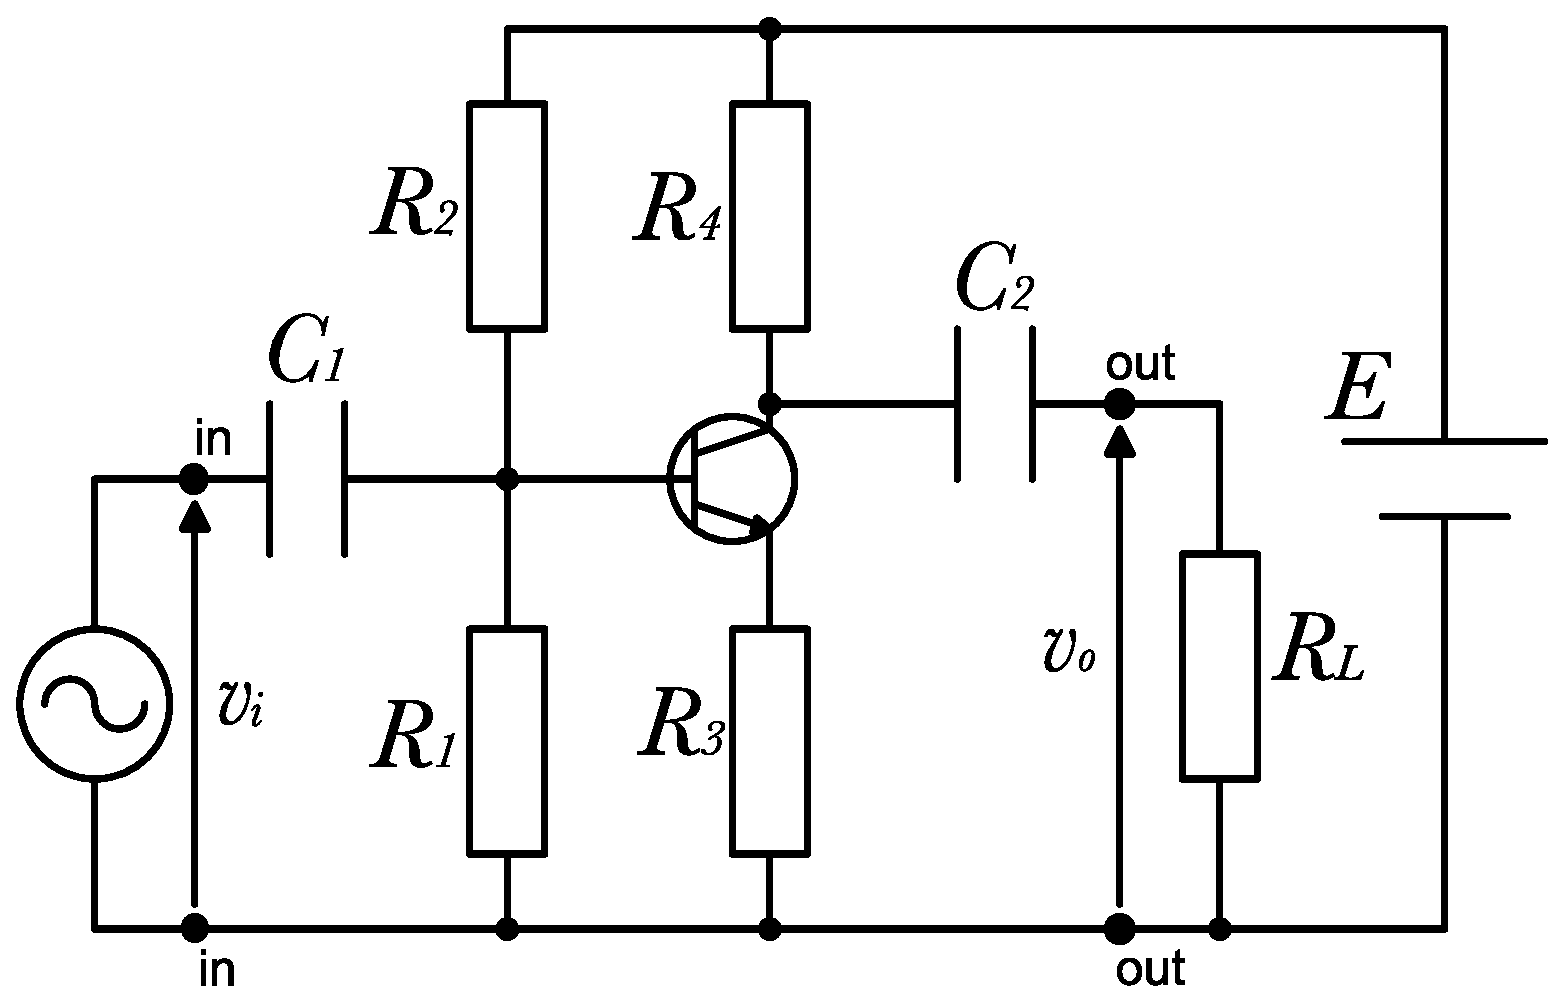
\includegraphics[width=0.7\hsize]{images/tr.eps}
        \caption{エミッタ増幅回路}
        \label{fig:tr}
    \end{figure}

    各定数: $R_1 = 22$ k$\Omega$, $R_2 = 100$ k$\Omega$, $R_3 = 2$ k$\Omega$, $R_4 = 10$ k$\Omega$,
    $R_L = 10$ k$\Omega$, $C_1 = 0.1$ $\mu$F, $C_2 = 10$ $\mu$F, $E = 15$ V

    使用トランジスタ: 2SC1815Y

    \subsection{増幅回路の理論特性}
        まず, この回路がどのような特性かを電気的等価回路から導かれる計算式を使って理論値を算出する.
        なお, 次に示す値は文献\cite{Text}付録Aのトランジスタ特性表から見積もったものを使用する.
        ($V_{BE} = 0.6 \mathrm{V}, h_{fe} = 180, h_{ie} = 4.2 \mathrm{k\Omega}$ ただし, $h_{oe} = 0, h_{re} = 0$とする).

        \subsubsection{バイアス値} \label{sssec:bias}
            \paragraph{バイアス回路を描き, 各電圧を算出する式を考えて, ベース端子の電圧$V_B$, コレクタ端子の電圧$V_C$, エミッタ端子の電圧$V_E$の各値を計算で求めよ. ($I_C >> I_B$と仮定して良い.)}
            \mbox{} \\

                バイアス回路を図\ref{fig:bias}に示す.

                \begin{figure}[h]
                    \centering
                    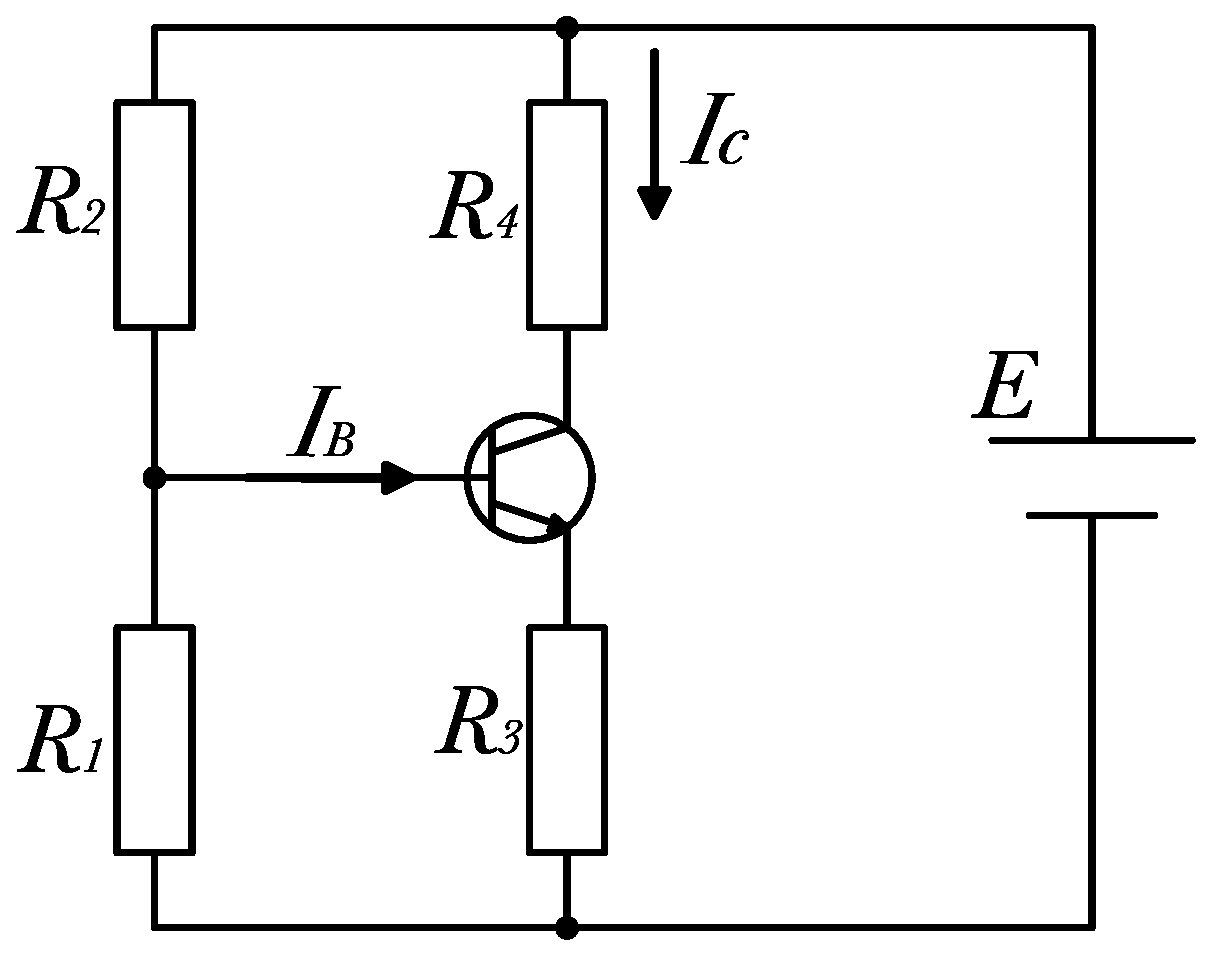
\includegraphics[width=0.6\hsize]{images/bias.eps}
                    \caption{バイアス回路}
                    \label{fig:bias}
                \end{figure}

                図より, $\displaystyle V_B = \frac{R_1}{R_1 + R_2} E$,
                $\displaystyle V_C = E - R_4I_C$,
                $V_E = V_B - V_{BE}$である.

                また, $\displaystyle I_C \approx I_E = \frac{V_E}{R_3}$とすると,
                $\displaystyle V_C = E - \frac{R_4}{R_3} V_E$となる.

                これらの式に値を代入して計算すると,
                $V_B \approx 2.7 \mathrm{V}, V_C \approx 4.5 \mathrm{V}, V_E \approx 2.1 \mathrm{V}$となる.

        \subsubsection{電圧利得} \label{sssec:gv}
            \paragraph{結合コンデンサ$C_1, C_2$のインピーダンスを無視した簡易等価回路を描き, 電圧増幅度$A_V$ [倍]を与える式を導出して電圧利得$G_V$ [dB]を計算で求めよ.}
            \mbox{} \\

                $C_1, C_2$のインピーダンスを無視した簡易等価回路を図\ref{fig:touka}に示す.

                \begin{figure}[h]
                    \centering
                    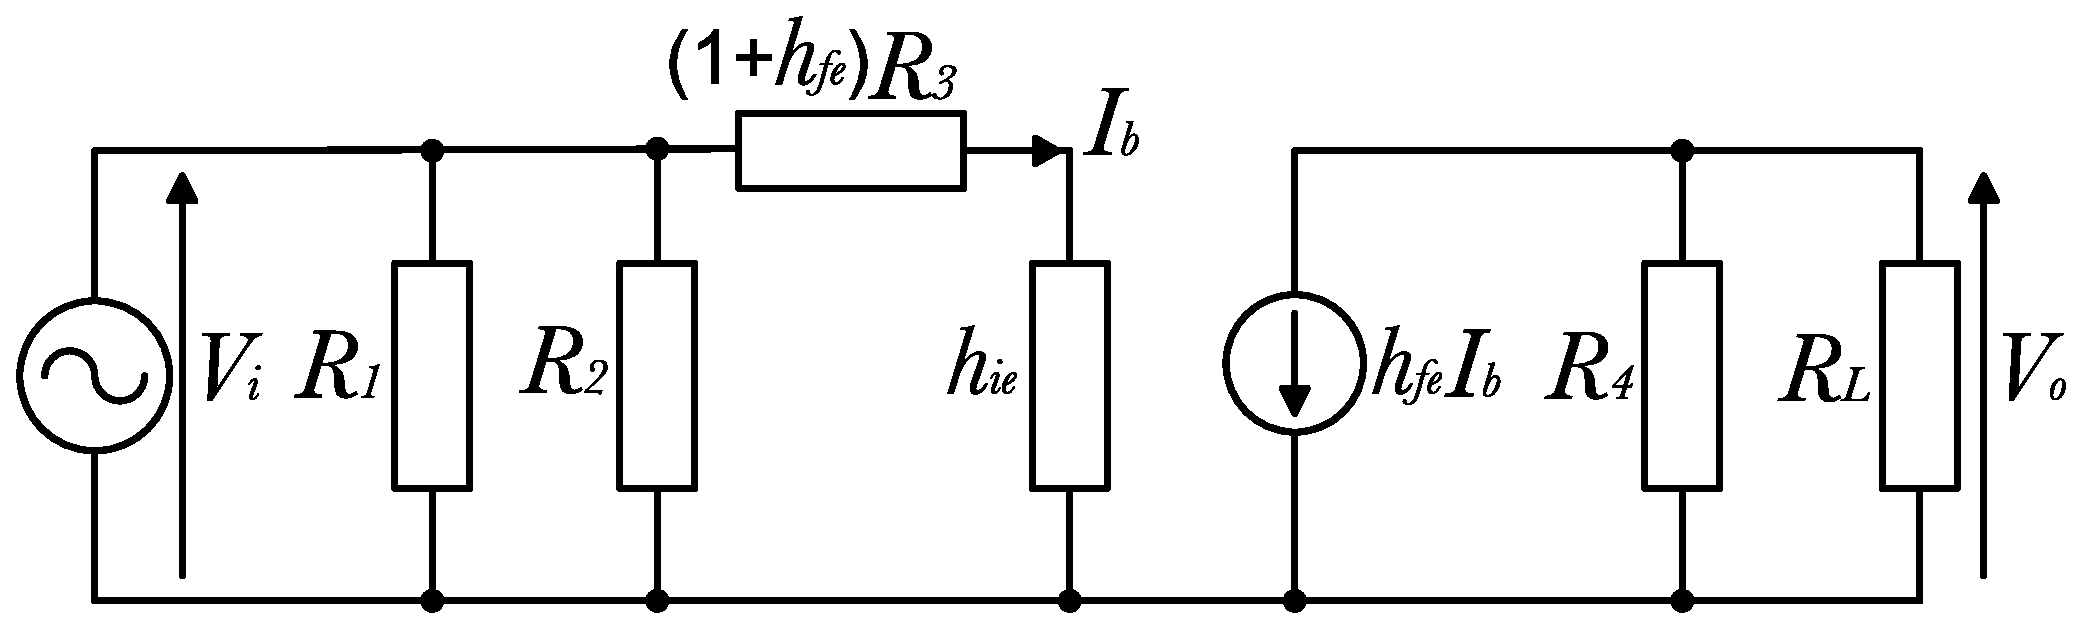
\includegraphics[width=1\hsize]{images/touka.eps}
                    \caption{$C_1, C_2$を除いた簡易等価回路}
                    \label{fig:touka}
                \end{figure}

                ここで, $V_i = \{h_{ie} + \left(1 + h_{fe}\right) R_3\}I_b$,
                $\displaystyle V_o = h_{fe}I_b\frac{R_4R_L}{R_4 + R_L}$となる.

                よって, $\displaystyle A_V = \frac{V_o}{V_i} = \frac{h_{fe}R_4R_L}{(R_4 + R_L)\{h_{ie} + (1 + h_{fe}) R_3\}} \approx 2.5$となる.
                また, $G_V = 20 \log_{10}{A_V} \approx 7.8 \mathrm{dB}$である.

        \subsubsection{低域カットオフ周波数} \label{sssec:cutoff}
            \paragraph{結合コンデンサ$C_2$のインピーダンスを無視し, $C_1$を含んだ簡易等価回路を描き, 低域のカットオフ周波数$f_L$を与える式を導出してその値を計算で求めよ.}
            \mbox{} \\

                $C_1$を含んだ簡易等価回路を図\ref{fig:touka1}に示す.

                \begin{figure}[h]
                    \centering
                    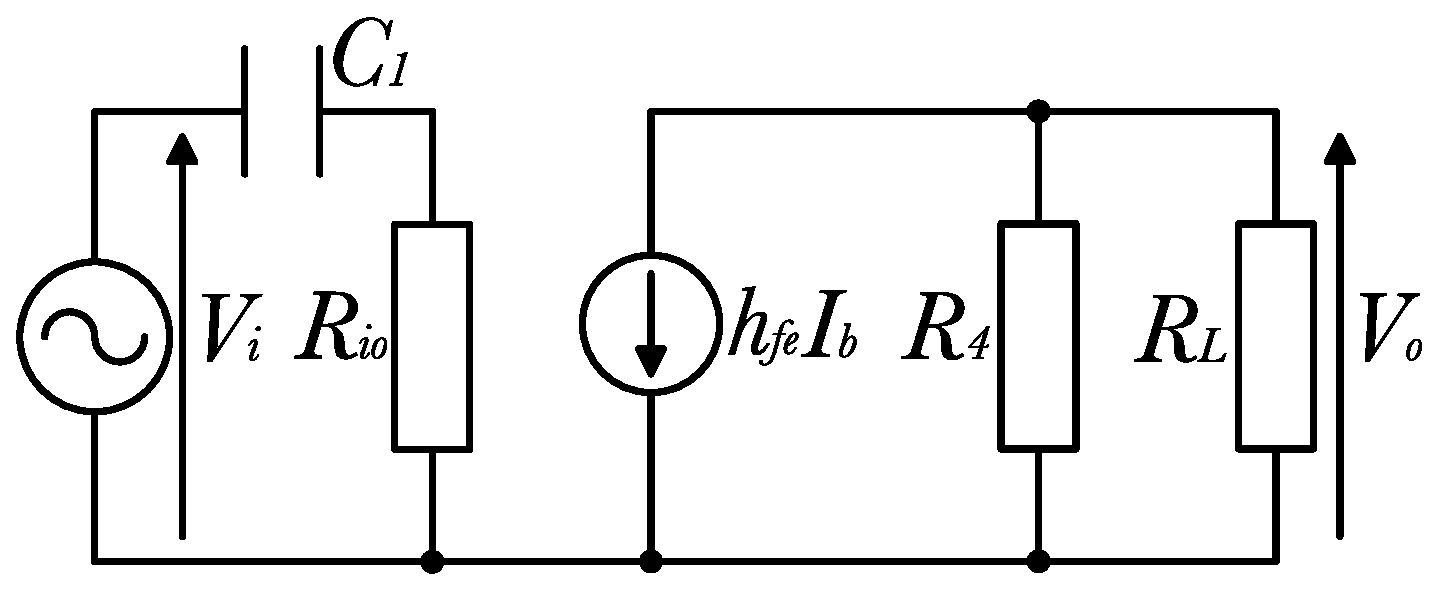
\includegraphics[width=0.7\hsize]{images/touka1.eps}
                    \caption{$C_2$を除いた簡易等価回路}
                    \label{fig:touka1}
                \end{figure}

                ここで, 入力側の$C_1$を除く負荷を$R_{io}$とまとめた.

                入力の周波数が$f_L$であるとき, 電圧利得は最大値の$\displaystyle\frac{1}{\sqrt{2}}$倍になる.
                $C_1$と$R_{io}$には同じ大きさの電流が流れるため,
                $R_{io}$による実部インピーダンスと$C_1$による虚部のインピーダンスの大きさは等しい.

                よって, このときの角周波数を$\omega$とすると,
                $\displaystyle\frac{1}{\omega C_1} = R_{io}$となる.
                $\omega = 2 \pi f_L$を代入して,
                $\displaystyle f_L = \frac{1}{2 \pi R_{io} C_1} \approx 93 \mathrm{Hz}$となる.

        \subsubsection{入力インピーダンス} \label{sssec:zi}
            \paragraph{結合コンデンサ$C_1, C_2$のインピーダンスを無視した簡易等価回路を描き, 入力インピーダンス$Z_i$を与える式を導出してその値を計算で求めよ.}
            \mbox{} \\

                簡易等価回路は, 図\ref{fig:touka}と同じようになる.
                入力インピーダンスは, 図\ref{fig:touka1}の$R_{io}$と等しくなるのでその大きさを求めると,
                $Z_i = R_{io} \approx 17 \mathrm{k\Omega}$となる.

        \subsubsection{出力インピーダンス} \label{sssec:zo}
            \paragraph{結合コンデンサ$C_1, C_2$のインピーダンスを無視した簡易等価回路を描き, 出力インピーダンス$Z_o$を与える式を導出してその値を計算で求めよ.}
            \mbox{} \\

                \ref{sssec:zi}と同じく, 簡易等価回路は図\ref{fig:touka}と等しくなる.

                よって, $Z_o = R_4 = 10 \mathrm{k\Omega}$となる.

        \subsubsection{出力波形の歪み} \label{sssec:distortion}
            \paragraph{入力電圧の振幅が増加すると, 出力波形がどのように歪むのか理論的に考えて説明せよ.}
            \mbox{} \\
                
                $v_{BE}$が入力電圧に応じて変化した時, $i_B$が0未満になる区間がある.
                そのとき, $I_B$は遮断されるため, その区間では$i_B = 0$となる.

                また, 同様に$i_B$が入力電圧に応じて変化した時, $v_{CE}$が0未満になる区間があり,
                $I_C$が飽和してしまう. そのため, その区間では$v_{CE} = 0$となる.

    \subsection{増幅回路の作成と実測}
        図\ref{fig:tr}に示す増幅回路(実験装置)を作成する.

        \subsubsection{バイアス電圧の測定}
            \paragraph{発振器の出力電圧を0Vとし, 次に示すバイアス電圧をデジタルマルチメータで測定せよ.} $V_B, V_C, V_E$
            \paragraph{\ref{sssec:bias}で求めた計算値と比較せよ.}
            \mbox{} \\

                測定した値と\ref{sssec:bias}で求めた計算値を表\ref{tab:bias}にまとめた.

                \begin{table}[h]
                    \caption{バイアス電圧}
                    \label{tab:bias}
                    \centering
                    \begin{tabular}{c||cc} \hline
                        & 計測値 [V] & 計算値 [V] \\ \hline
                        $V_B$ & 2.6 & 2.7 \\
                        $V_C$ & 5.5 & 4.5 \\
                        $V_E$ & 2.0 & 2.1 \\ \hline
                    \end{tabular}
                \end{table}

                $V_B$, $V_E$にはほとんど誤差が現れていないが, $V_C$には1Vの誤差がみて取れる.
                \ref{sssec:bias}の式をみると, $V_E$の誤差が$\displaystyle\frac{R_3}{R_4}$倍されて$V_C$
                に現れることがわかる. よって, $V_C$に比較的大きな誤差が現れていると考えられる.

        \subsubsection{電圧利得の測定}
            入力端子にDMM1(交流電圧レンジ)とオシロスコープのCH1を接続し,
            出力端子にDMM2(交流電圧レンジ)とオシロスコープのCH2を接続する.
            DMMの表示は実効値(rms)で表示されるので注意する.

            \paragraph{発振器の周波数と電圧をそれぞれ$f = 10$ kHz, $V_i = 0.4 \mathrm{V_{rms}}$とし, 入出力波形をオシロスコープで観察し(ch1: $v_i$, ch2: $v_o$), 画像を記録せよ.}
            \paragraph{オシロスコープで読み取った入出力電圧の振幅値と, 2台のデジタルマルチメータで読み取った入出力電圧の実効値を表にまとめて, それらの関係が正しいことを確認し, この時の電圧増幅度$A_V$ [倍]及び電圧利得$G_V$ [dB]はいくらになるか求めよ.}
            \paragraph{\ref{sssec:gv}で求めた計算値と比較せよ.}
            \mbox{} \\

                $f = 10$ kHz, $V_i = 0.4 \mathrm{V_{rms}}$としたときの入出力波形を図\ref{fig:oscillo}に示す.

                \begin{figure}[h]
                    \centering
                    \includegraphics[width=0.55\hsize]{images/AB_2-2-2_04V0p.jpg}
                    \caption{入出力波形($f = 10$ kHz, $V_i = 0.4 \mathrm{V_{rms}}$)}
                    \label{fig:oscillo}
                \end{figure}

                オシロスコープの画面から読み取れる振幅値と, DMMで読み取った振幅値を表\ref{tab:amp}にまとめる.

                \begin{table}[h]
                    \caption{入出力電圧}
                    \label{tab:amp}
                    \centering
                    \begin{tabular}{c||cc} \hline
                        & オシロスコープ計測値 [mV] & デジタルマルチメータ計測値 [mVrms] \\ \hline
                        $V_i$ & 350 & 236 \\
                        $V_o$ & 830 & 590 \\ \hline
                    \end{tabular}
                \end{table}

                表より, デジタルマルチメータ計測値を$\sqrt{2}$倍するとほぼ値が等しいことがわかる.

                次に, 表\ref{tab:av}にオシロスコープとDMMで計測した電圧増幅度と電圧利得と,
                \ref{sssec:gv}で求めた理論値をまとめる.

                \begin{table}[h]
                    \caption{電圧増幅度と電圧利得}
                    \label{tab:av}
                    \centering
                    \begin{tabular}{c||ccc} \hline
                        & オシロスコープ & デジタルマルチメータ & 理論値 \\ \hline
                        $A_V$ [倍] & 2.37 & 2.51 & 2.5 \\
                        $G_V$ [dB] & 7.49 & 7.96 & 7.8 \\ \hline
                    \end{tabular}
                \end{table}

                表から, おおよそ理論値と値が等しいことがわかる.

        \subsubsection{増幅率の周波数特性}
            \paragraph{発振器の電圧$V_i$を0.4V一定とし, 発振器の周波数$f$を10Hz, 20Hz, 50Hz, 100Hz, 200Hz$\cdots$100kHzとしたときの出力電圧$V_o$の実効値を測定し, 電圧利得$G_V$を求める.(発振器の周波数を変化させると, 発振器の出力電圧も変化する場合があるので注意すること.)$f, V_i, V_o, G_V$の関係を表にまとめよ.}
            \paragraph{横軸を$f$, 縦軸を$G_V$として片対数グラフにプロットせよ.}
            \paragraph{電圧利得が最大利得より3dB低下する周波数(カットオフ周波数)$f_L$はどれくらいかグラフより求めよ.($f_L$付近では発振器の周波数$f$をより細かく変化させ, データを取る事).}
            \paragraph{\ref{sssec:cutoff}で求めた計算値と比較せよ.}
            \mbox{} \\
                
                測定結果を表\ref{tab:amp}, 片対数グラフを図\ref{fig:amp}に示す.

                \begin{table}[h]
                    \caption{周波数特性}
                    \label{tab:amp}
                    \centering
                    \begin{tabular}{ccc||ccc} \hline
                        $f$ [Hz] & $V_o$ [mVrms] & $G_V$ [dB] & $f$ [kHz] & $V_o$ [Vrms] & $G_V$ [dB] \\ \hline
                        10 & 122 & -7.31 & 0.2 & 0.882 & 9.87 \\
                        20 & 224 & -2.03 & 0.5 & 0.955 & 10.6 \\
                        50 & 483 & 4.64 & 1 & 0.977 & 10.8 \\
                        60 & 545 & 5.69 & 2 & 0.986 & 10.8 \\
                        70 & 606 & 6.61 & 5 & 0.997 & 10.9 \\
                        80 & 656 & 7.30 & 10 & 1.012 & 11.1 \\
                        90 & 693 & 7.78 & 20 & 1.019 & 11.1 \\
                        100 & 723 & 8.15 & 50 & 1.018 & 11.1 \\
                        120 & 778 & 8.78 & 100 & 0.895 & 10.0 \\
                        150 & 831 & 9.36 & & & \\ \hline
                    \end{tabular}
                \end{table}

                \begin{figure}[h]
                    \centering
                    \includegraphics[width=0.7\hsize]{images/amp.png}
                    \caption{周波数特性}
                    \label{fig:amp}
                \end{figure}

                表より, $G_V$の最大値は8.12 dBである. よって, 約5.12dBの100Hz付近が$f_L$であると読み取れる.
                \ref{sssec:cutoff}で求めた計算値は93Hzであったが,
                計算値を出す過程で特性表より特性値を見積もっているために誤差が生まれたと考えられる.

        \subsubsection{入力インピーダンスの測定}
            \begin{figure}[H]
                \begin{minipage}{0.6\hsize}
                    \paragraph{図\ref{fig:tr_zi}のように$R_R$ = 10k$\Omega$の抵抗を接続し, 発振器の周波数を$f$ = 10kHz, 電圧を$V_s$ = 0.4Vrmsとする.$V_s$及び$V_i$の各電圧をDMMで測定し, (\ref{equ:zi})式より入力インピーダンス$Z_i$を求めよ.}
                    
                    \begin{equation}
                        Z_i = \frac{V_i}{V_s - V_i} R_R \label{equ:zi}
                    \end{equation}
                \end{minipage}
                \begin{minipage}{0.4\hsize}
                    \centering
                    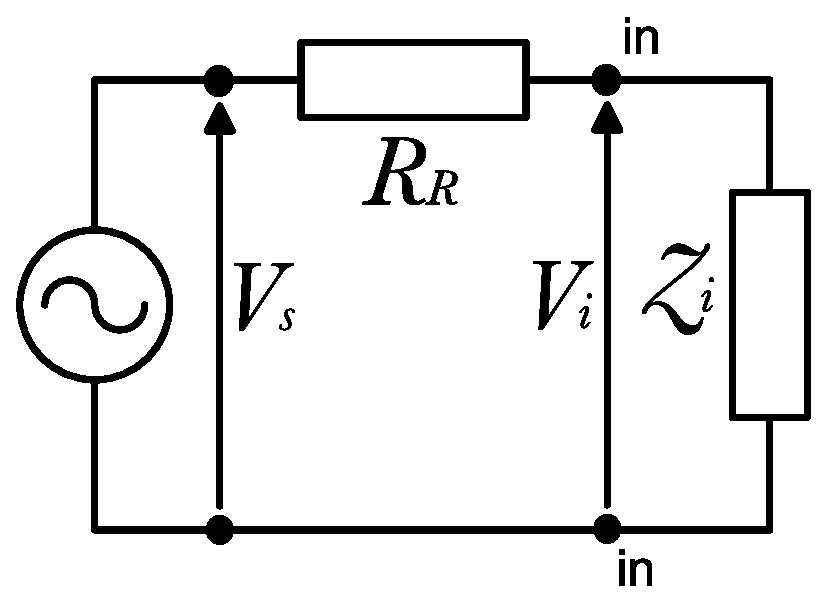
\includegraphics[width=0.72\hsize]{images/tr_zi.eps}
                    \caption{入力インピーダンス測定回路}
                    \label{fig:tr_zi}
                \end{minipage}
            \end{figure}

            \paragraph{\ref{sssec:zi}で求めた計算値と比較せよ.}
            \mbox{} \\

                値を計測すると, $V_i = 0.239$ Vrmsとなった.
                式に代入して計算すると, $Z_i \approx 14.8$k$\Omega$となる.
                \ref{sssec:zi}で求めた値は17k$\Omega$であった.
                この誤差は, $f_L$に生じたものと同様に特性値からきたものだと考えられる.

        \subsubsection{出力インピーダンスの測定}
            \paragraph{図\ref{fig:tr_zo}で発振器の周波数を$f$ = 10kHz, 電圧を$V_i$ = 0.4Vrmsとする. SWを開いた時($R_L$をはずした時)の出力端電圧$V_{oo}$とSWを閉じた時($R_L$を接続した時)の電圧$V_o$をDMMで測定し, (\ref{equ:zo})式より出力インピーダンス$Z_o$を求めよ.}

            \begin{figure}[h]
                \centering
                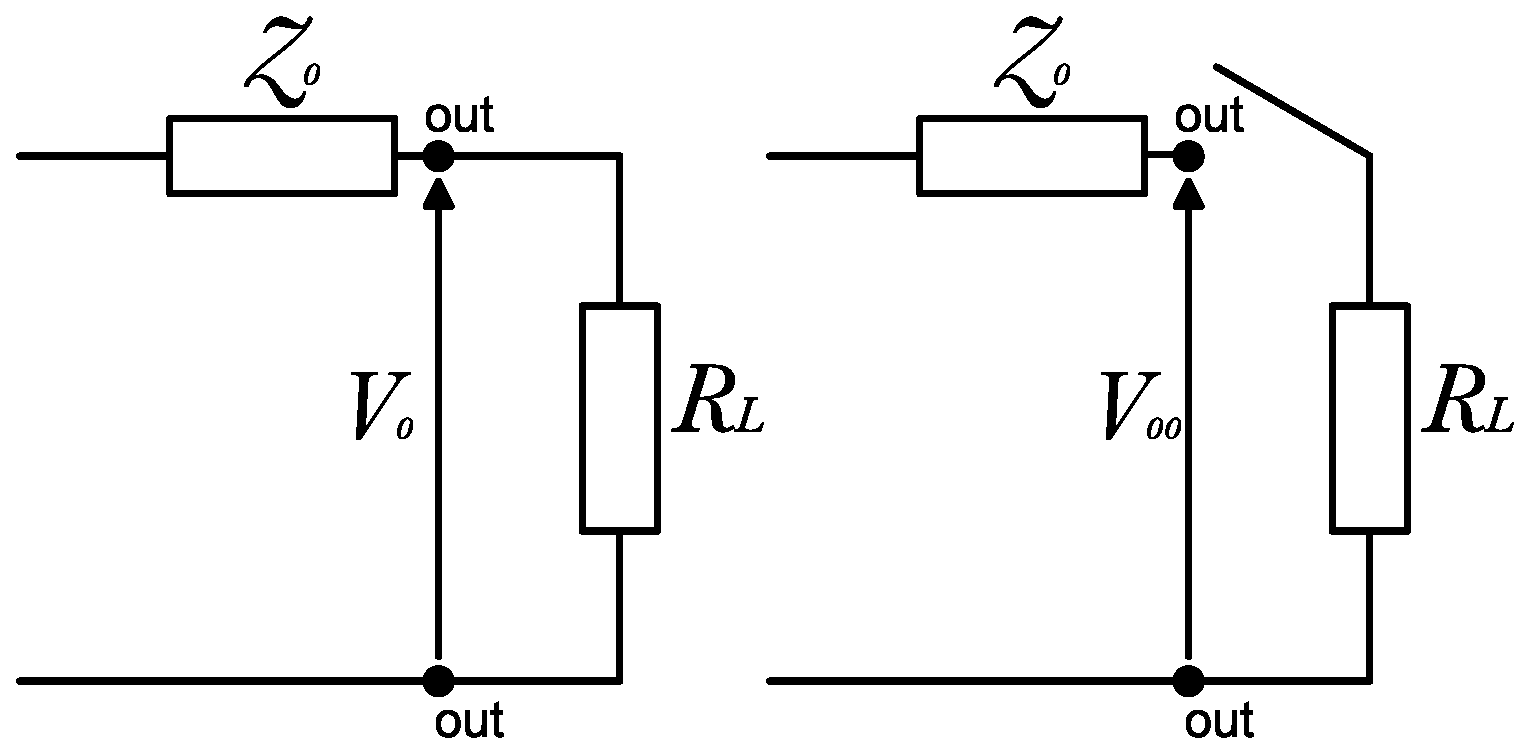
\includegraphics[width=0.75\hsize]{images/tr_zo.eps}
                \caption{出力インピーダンス測定回路}
                \label{fig:tr_zo}
            \end{figure}

            \begin{equation}
                Z_o = \frac{V_{oo} - V_o}{V_o} R_L \label{equ:zo}
            \end{equation}

            \paragraph{\ref{sssec:zo}で求めた計算値と比較せよ.}
            \mbox{} \\

                測定した結果, $V_oo = 0.973 \mathrm{V}, V_o = 1.95 \mathrm{V}$となった.
                式に代入して計算をすると, $Z_o \approx 10 \mathrm{k\Omega}$となり,
                \ref{sssec:zo}で求めた値とほぼ等しい値になることがわかる.

        \subsubsection{増幅率の測定と波形歪みの観測}
            \paragraph{図\ref{fig:tr}で発振器の周波数を$f$ = 10kHzに固定とする. 入力電圧$V_i$を0.1Vrms, 0.2Vrms, 0.3Vrms $\cdots$と上昇させた時の出力電圧値$V_o$をDMMで測定していく(オシロスコープで出力端電圧波形を観察し, 波形に歪みが生じるまで測定する). 出力波形に歪みが生じ始めるのは入力電圧がどれくらいの時か測定せよ.}
            \paragraph{入力電圧$V_i$ = 1.0Vrms時の入力波形と出力波形をオシロスコープで同時観察し(ch1: $v_i$, ch2: $v_o$), 画像を記録せよ.}
            \paragraph{\ref{sssec:distortion}で考えた波形と比較せよ.}
            \mbox{} \\

                測定した結果, $V_i =  0.717$ Vrmsの時に波形が歪み出した.
                $V_i = 1.0$ Vrmsのときの波形画像を図\ref{fig:hzm}に示す.

                \begin{figure}[h]
                    \centering
                    \includegraphics[width=0.7\hsize]{images/AB_2-2-6_1Vrms.jpg}
                    \caption{歪んだ出力波形}
                    \label{fig:hzm}
                \end{figure}

                図を見ると, 出力波形の下部分だけが歪んでいる.
                これは, ベース電流の遮断のみが起きているからであると考えられる.

\section{R-L-C共振回路とその特性}
    \begin{figure}[H]
        \begin{minipage}{0.6\hsize}
            ここでは, 抵抗, コイル, コンデンサより構成されるR-L-C直列共振回路を取り上げ,
            そのアドミッタンス特性と回路定数の算出方法について学ぶ.
            図\ref{fig:rlc}はR-L-C直列回路に交流電源を接続したものである.
            この回路のアドミッタンス周波数特性は図\ref{fig:admittance_hz}のようになり,
            アドミッタンスループ特性は図\ref{fig:admittance_loop}のようになる.
            ここで, 電源の角周波数を$\omega$とする($\omega = 2 \pi f$).
        \end{minipage}
        \begin{minipage}{0.4\hsize}
            \centering
            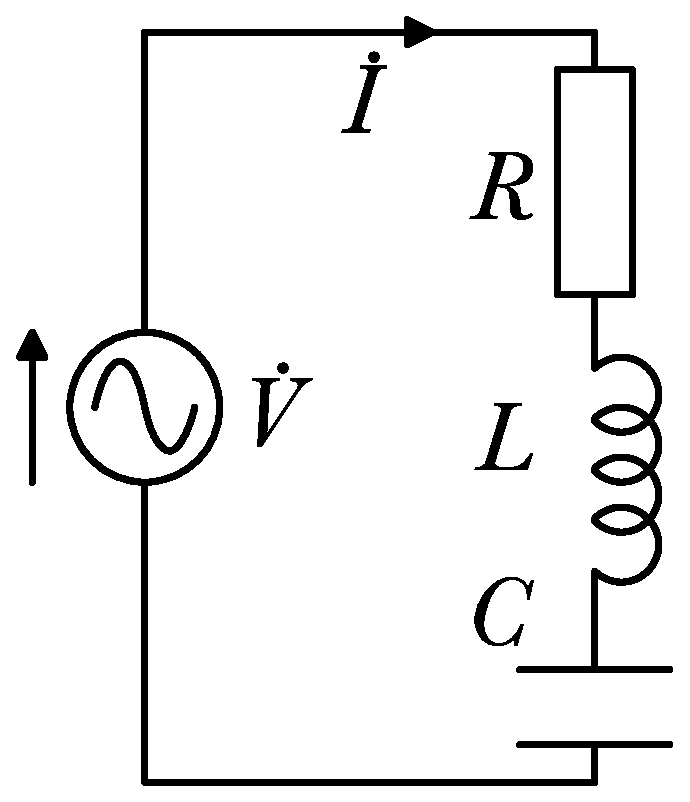
\includegraphics[width=0.6\hsize]{images/rlc.eps}
            \caption{R-L-C直列回路}
            \label{fig:rlc}
        \end{minipage}
    \end{figure}

    \begin{figure}[h]
        \begin{minipage}{0.5\hsize}
            \centering
            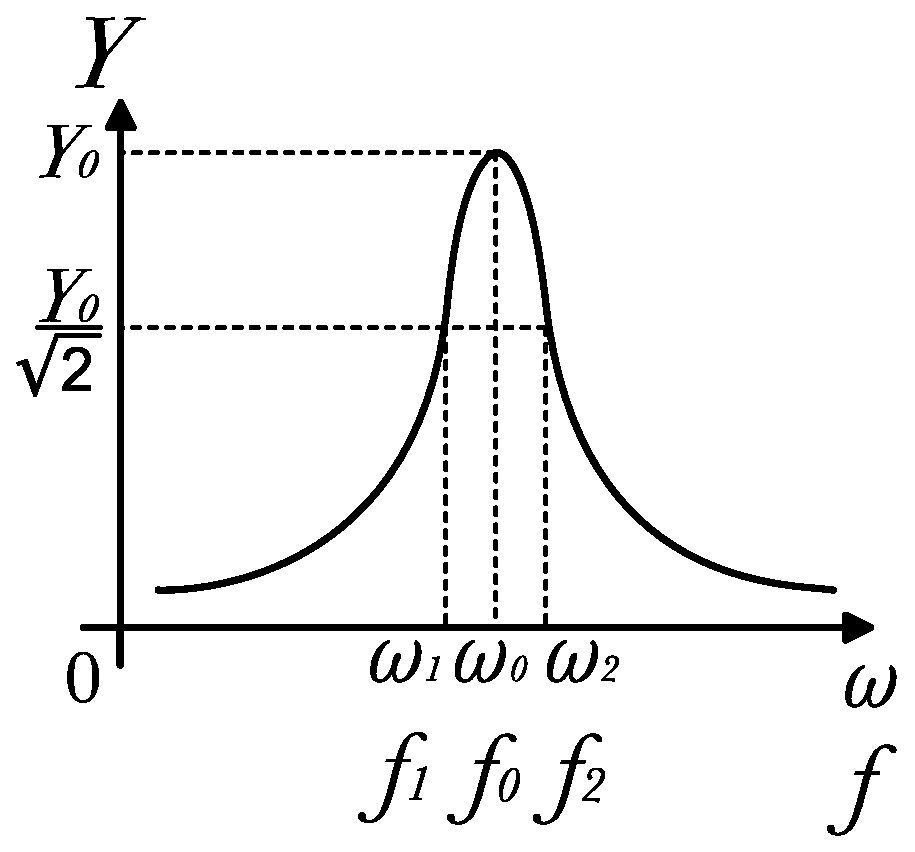
\includegraphics[width=0.8\hsize]{images/admittance.eps}
            \caption{アドミッタンスの周波数特性}
            \label{fig:admittance_hz}
        \end{minipage}
        \begin{minipage}{0.5\hsize}
            \centering
            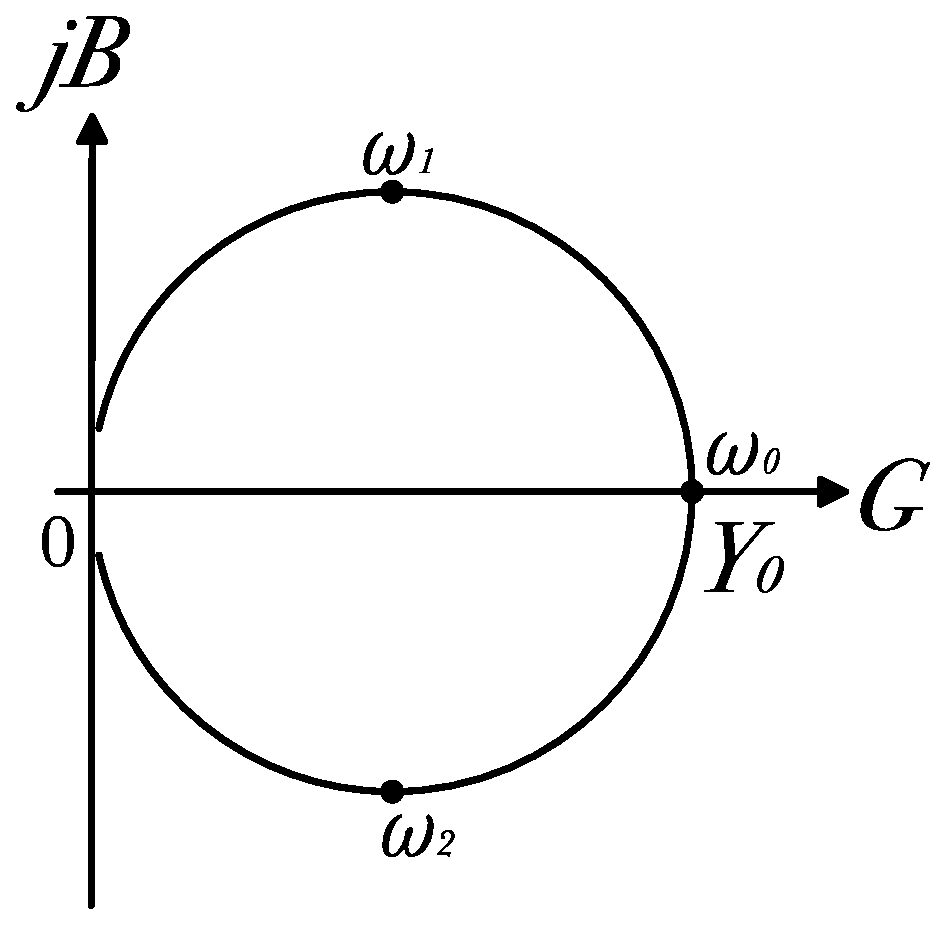
\includegraphics[width=0.8\hsize]{images/admittance_loop.eps}
            \caption{アドミッタンスループ特性}
            \label{fig:admittance_loop}
        \end{minipage}
    \end{figure}

    \subsection{定数と理論特性}
        \subsubsection{アドミッタンスと共振周波数}
            \paragraph{図\ref{fig:rlc}において, 電源の角周波数を$\omega$とし, 複素アドミッタンス$\dot{Y}$とその大きさ$Y$を与える式を示せ.また, アドミッタンスの大きさ$Y$が最大(共振)となるときの角共振周波数$\omega_0$の値と, その時の$\dot{Y}$の大きさ$Y_0$を与える式を導出せよ.}
            \mbox{} \\

                回路の複素インピーダンスを$\dot{Z}$とすると,
                $\displaystyle\dot{Y} = \frac{1}{\dot{Z}}$となる.

                よって, $\displaystyle\dot{Y} = \frac{1}{\dot{Z}} = \frac{1}{R + j(\omega L - \frac{1}{\omega C})}$,
                $\displaystyle Y = \frac{1}{Z} = \frac{1}{\sqrt{R^2 + (\omega L - \frac{1}{\omega C})^2}}$となる.

                $Y$が最大となる時, $\displaystyle \omega L = \frac{1}{\omega C}$となるので,
                $\displaystyle\omega_0 = \frac{1}{\sqrt{LC}}$となる.

                また, $\displaystyle\omega L - \frac{1}{\omega C} = 0$なので, $\displaystyle Y_0 = \frac{1}{R}$となる.

        \subsubsection{アドミッタンスループ}
            \paragraph{複素インピーダンスを$\dot{Z} = R + jX (R: レジスタンス, X: リアクタンス)$, 複素アドミッタンスを$\dot{Y} = G + jB (G: コンダクタンス, B: サセプタンス)$としたとき, $\displaystyle\dot{Z} = \frac{1}{\dot{Y}}$の関係から, アドミッタンス軌跡(横軸$G$, 縦軸$B$)は$\displaystyle\left(\frac{1}{2R}, 0\right)$を中心とし, 半径$\displaystyle\frac{1}{2R}$の円を描くことを示せ.}
            \mbox{} \\

                仮定より, $\displaystyle R + jX = \frac{1}{G + jB} = \frac{G - jB}{G^2 + B^2}$
                
                実部に注目して,
                
                \begin{eqnarray*}
                    &&R = \frac{G}{G^2 + B^2} \\
                    &&\leftrightarrow G^2 + B^2 - \frac{G}{R} = 0 \\
                    &&\leftrightarrow G^2 - \frac{G}{R} + \left(\frac{1}{2R}\right)^2 + B^2 = \left(\frac{1}{2R}\right)^2 \\
                    &&\leftrightarrow \left(G - \frac{1}{2R}\right)^2 + B^2 = \left(\frac{1}{2R}\right)^2
                \end{eqnarray*}

                上式より, アドミッタンス軌跡は$\displaystyle\left(\frac{1}{2R}, 0\right)$を中心とし,
                半径$\displaystyle \frac{1}{2R}$の円を描くことがわかる.

        \subsubsection{品質係数$Q$値の算出} \label{sssec:q}
            \paragraph{共振時では, $\displaystyle\omega_0L = \frac{1}{\omega_0C}$となる. ここで, 両辺を$R$で割り, 品質係数$Q$を$\displaystyle Q = \frac{\omega_0L}{R} = \frac{1}{\omega_0CR}$と定義する. 図\ref{fig:admittance_hz}, \ref{fig:admittance_loop}で, $\displaystyle Y = \frac{Y_0}{\sqrt{2}}$を与える角周波数を$\omega_2, \omega_1$とするとき($\omega_1 < \omega_2$で, $\omega_1, \omega_2$はそれぞれ$B$最大値と$B$最小値を与える角周波数), $\displaystyle Q = \frac{\omega_0}{\omega_2 - \omega_1}$となる関係式を導き出せ.}
            \mbox{} \\
                
                $\displaystyle Y = \frac{Y_0}{\sqrt{2}} = \frac{1}{\sqrt{2}R}$より,
                $\displaystyle 2R^2 = Z^2 = R^2 + (\omega L - \frac{1}{\omega C})^2 \leftrightarrow \pm R = \omega L - \frac{1}{\omega C}$

                これを$\omega$について解くと,
                $\displaystyle\omega = \frac{\pm RC \pm \sqrt{R^2C^2 + 4LC}}{2LC}$

                $RC - \sqrt{R^2C^2 + 4LC} <= 0$なので, 解として適さない.

                よって, $\omega_1 < \omega_2$より,
                $\displaystyle \omega_1 = \frac{-RC + \sqrt{R^2C^2 + 4LC}}{2LC}$,
                $\displaystyle \omega_2 = \frac{RC + \sqrt{R^2C^2 + 4LC}}{2LC}$となる.

                これらを$\displaystyle Q = \frac{\omega_0}{\omega_2 - \omega_1}$に代入すると,
                $\displaystyle Q = \frac{\omega_0 L}{R}$となる.

        \subsubsection{$R$, $L$, $C$値の算出方法} \label{sssec:rlc}
            \paragraph{R, L, Cの値がわからないとき, アドミッタンスループ特性より$Y_0, \omega_0, \omega_2, \omega_1$を測定すれば, 以下の式より, $R, L, C$の値を算出することができる. それぞれの式を導き出せ.}
            \mbox{} \\
                
                \begin{eqnarray*}
                    R &=& \frac{1}{Y_0} \\
                    L &=& \frac{Q}{\omega_0 Y_0} \\
                    C &=& \frac{Y_0}{\omega_0 Q}
                \end{eqnarray*}
            
                $\displaystyle Y_0 = \frac{1}{R}$より,
                $\displaystyle R = \frac{1}{Y_0}$

                \ref{sssec:q}より,
                \begin{eqnarray*}
                    Q &=& \frac{\omega_0L}{R} = \omega_0 L Y_0 \\
                    Q &=& \frac{1}{\omega_0CR} = \frac{Y_0}{\omega_0C} \\
                \end{eqnarray*}
                
                これらをそれぞれ$L, C$について解くと,
                $\displaystyle L = \frac{Q}{\omega_0 Y_0}, C = \frac{Y_0}{\omega_0 Q}$となる.
            

    \subsection{R-L-C回路のアドミッタンス特性測定と定数の算出}
        \subsubsection{アドミッタンス特性の測定}
            \begin{figure}[h]
                \begin{minipage}{0.6\hsize}
                    \paragraph{図\ref{fig:rlc_exp}に示すようにR-L-C直列回路にLCRメータを接続し, アドミッタンスの周波数特性及びアドミッタンスループ特性を測定し, その数値データを使ってそれぞれグラフ化し提示せよ. このとき, 掃引周波数範囲及び周波数の分解能は任意とする.}

                    \mbox{}

                \end{minipage}
                \begin{minipage}{0.4\hsize}
                    \centering
                    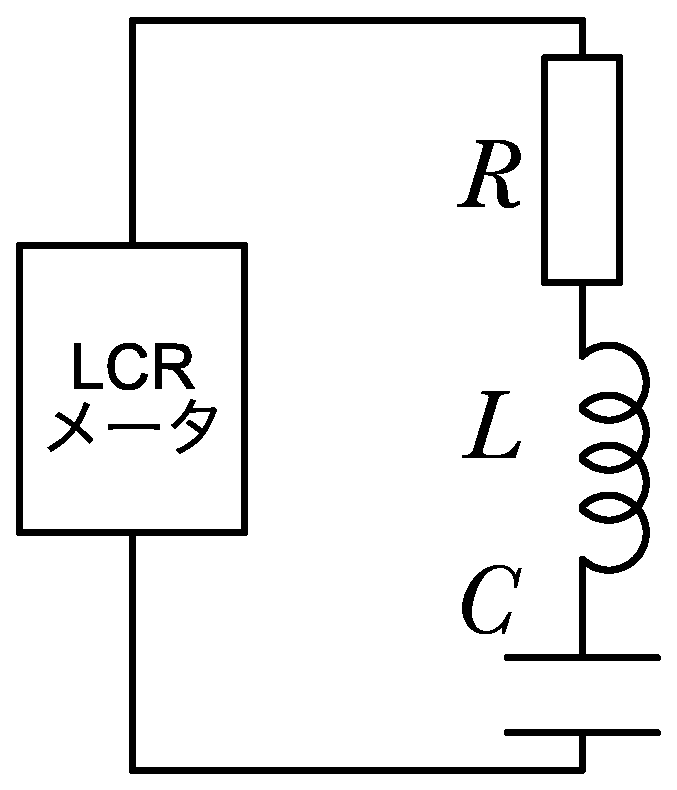
\includegraphics[width=0.6\hsize]{images/exp.eps}
                    \caption{入力インピーダンス測定回路}
                    \label{fig:rlc_exp}
                \end{minipage}
            \end{figure}

            \paragraph{実験データより, $Y_0, f_0, f_2, f_1 (\omega_0, \omega_2, \omega_1)$の値を求めよ.}
            \mbox{} \\

                グラフをそれぞれ図\ref{fig:amp2}, \ref{fig:loop}に示す.

                \begin{figure}[h]
                    \begin{minipage}{0.5\hsize}
                        \centering
                        \includegraphics[width=1\hsize]{images/amp2.png}
                        \caption{アドミッタンスの周波数特性}
                        \label{fig:amp2}
                    \end{minipage}
                    \begin{minipage}{0.5\hsize}
                        \centering
                        \includegraphics[width=0.9\hsize]{images/loop.png}
                        \caption{アドミッタンスループ特性}
                        \label{fig:loop}
                    \end{minipage}
                \end{figure}

                実験データより, $Y_0 = 35.7 \mathrm{mS}, f_0 \approx 7675 \mathrm{Hz}$である.
                アドミッタンスが$\displaystyle\frac{Y_0}{\sqrt{2}} \approx 25.2 \mathrm{mS}$となる周波数を求めると,
                $f_1 \approx 7450 \mathrm{Hz}, f_2 \approx 7920 \mathrm{Hz}$となる.

                $\omega = 2 \pi f$に各値を代入すると,
                $\omega_0 \approx 4820 \times 10$ rad/s,
                $\omega_1 \approx 4679 \times 10$ rad/s,
                $\omega_2 \approx 4974 \times 10$ rad/sとなる.

        \subsubsection{定数の算出}
            \paragraph{\ref{sssec:q}, \ref{sssec:rlc}から, $Q, R, L, C$の値を算出せよ.}
            \mbox{} \\

                各値を求めると,

                \begin{eqnarray*}
                    Q &=& \frac{\omega_0}{\omega_2 - \omega_1} \approx 16.2 \\
                    R &=& \frac{1}{Y_0} \approx 28.0 \ \mathrm{\Omega} \\
                    L &=& \frac{Q}{\omega_0 Y_0} \approx 9.41 \ \mathrm{mH} \\
                    C &=& \frac{Y_0}{\omega_0Q} \approx 45.7 \ \mathrm{nF}
                \end{eqnarray*}

                となる.

        \subsubsection{グラフの追記}
            \paragraph{求めた等価回路定数を使って, アドミッタンスの周波数特性及びアドミッタンスのループ円を計算し, 実測したグラフに追記し, 新たに提示しなさい.}
            \mbox{} \\

                $\displaystyle Y = \frac{1}{\sqrt{R^2 + \left(\omega L - \frac{1}{\omega C}\right)^2}}$
                に値を代入して, $\displaystyle Y \approx \frac{1}{\sqrt{784 + \left(5.91 \times 10^{-2} f - \frac{1}{2.87 \times 10^{-7} f}\right)^2}}$ [S]となる.

                また, $\displaystyle \left(G - \frac{1}{2R}\right)^2 + B^2 = \left(\frac{1}{2R}\right)^2$
                に値を代入して, $\displaystyle \left(G - 1.785 \times 10^{-2}\right)^2 + B^2 = 3.189 \times 10^{-4}$となる.
                
                これらの式を図\ref{fig:amp2}, \ref{fig:loop}に追加でプロットしたものを図\ref{fig:amp3}, \ref{fig:loop2}に示す.

                \begin{figure}[h]
                    \begin{minipage}{0.5\hsize}
                        \centering
                        \includegraphics[width=1\hsize]{images/amp3.png}
                        \caption{アドミッタンスの周波数特性}
                        \label{fig:amp3}
                    \end{minipage}
                    \begin{minipage}{0.5\hsize}
                        \centering
                        \includegraphics[width=0.9\hsize]{images/loop2.png}
                        \caption{アドミッタンスループ特性}
                        \label{fig:loop2}
                    \end{minipage}
                \end{figure}

                それぞれのグラフの線がほぼ被っていることから, 理論通りの結果が得られていることがわかる.

\section{課題}
    \subsection{エミッタ接地, ベース接地, コレクタ接地の各増幅回路の特徴についてまとめよ.}
        それぞれの増幅回路の特徴を表\ref{tab:feature}にまとめる.

        \begin{table}[h]
            \caption{増幅回路の特徴}
            \label{tab:feature}
            \centering
            \begin{tabular}{c||ccc} \hline
                & エミッタ接地 & コレクタ接地 & ベース接地 \\ \hline
                入力インピーダンス & 低い & 高い & 低い \\
                出力インピーダンス & 高い & 低い & 高い \\
                電圧利得 & 大きい & 約1 & 大きい \\
                電流利得 & 大きい & 大きい & 約1 \\
                周波数特性 & 悪い & 良い & 良い \\ \hline
            \end{tabular}
        \end{table}

        表より, エミッタ接地回路が電圧も電流も増幅するのに対し,
        コレクタ接地回路とベース接地回路は片方ずつしか増幅をしないことがわかる.
        これに伴い, 電力増幅度もエミッタ増幅接地回路は他の二つの回路よりも高くなる.

        エミッタ接地回路, ベース接地回路とコレクタ接地回路には入出力インピーダンスの違いもある.

        また, エミッタ接地回路とベース接地回路, コレクタ接地回路には周波数特性の違いがある.
        これは, 回路中のキャパシタによるインピーダンスが影響しているためである.
        これらの違いをうまく使い分ける必要がある.

    \subsection{共振回路の応用用途にはどのようなものがあるか調査し, それぞれについてまとめよ.}
        共振回路が用いられている例として, ラジオがある.
        ラジオの内部にある共振回路のインダクタンスやキャパシタンスを変更することで共振する周波数を選択し,
        放送局を選択することができる. この回路は同調回路と呼ばれる.

        もう一つの応用例として, 盧波器がある.
        盧波器は, フィルタ回路とも呼ばれ, 内部に共振回路があり,
        共振周波数付近の信号のみを取り出すことが可能になっている.

\section{感想}
    代表者による実験だったため,
    自分が手を動かすことはほぼなかったが,
    しっかりと内容の理解をすることができたと思う.

    レポートの内容として,
    文量は今までのレポートよりも多いものの,
    考える必要のある部分はそう多くなく,
    あまり苦労せずに終えることができた.
    次の実験も予習をしっかりして望みたい.

\begin{thebibliography}{99}
    \bibitem{Support Page} Ec4電子制御工学実験 https://www2.st.nagaoka-ct.ac.jp/
    \bibitem{Text} トランジスタの増幅回路とR-L-C共振回路 Ver.2020, 令和2年$\cdot$前期実験テキスト
    \bibitem{} トランジスタ増幅回路の接地方式ごとの、電流・電力増幅度の比較 - 無線工学の基礎 \\ http://www.gxk.jp/elec/musen/1ama/H16/html/H1604A07\_.html
    \bibitem{} エミッタ接地回路、コレクタ接地回路、ベース接地回路の違い - Electrilcal Information \\ https://detail-infomation.com/difference-of-amplifier-circuit/
    \bibitem{} 直列共振回路が用いられている例 - 大阪電気通信大学松浦研究室 \\ http://www.osakac.ac.jp/labs/matsuura/japanese/lesson/ElectricCircuit/AlternativeCircuit/\\ExampleOfSeriesResonanceCircuit.pdf
    \bibitem{} 「フィルタ回路」の解説 - しなぷすのハード製作記 \\ https://synapse.kyoto/glossary/filter/page001.html
\end{thebibliography}

\end{document}
